% !TEX encoding = UTF-8
% !TEX program = lualatex

\documentclass[a4paper]{article}

\usepackage[left=1.5cm, right=1.5cm, top=1cm, bottom=2cm]{geometry}

\usepackage{mathtools, amssymb}
    \def\CC{\mathbf C}
    \def\DD{\mathbf D}
    \def\RR{\mathbf R}

\usepackage[no-math]{fontspec}
    \setmainfont{Noto Serif}
    \setsansfont{Noto Sans TC}
    \setmonofont{Noto Sans Mono}

\usepackage{tikz}

\begin{document}

\parindent 0pt
\parskip 1em

\newcounter{prblm}
\def\Problem{\stepcounter{prblm}[\theprblm] }

\section*{Complex Variable - Midterm Exam}

\sffamily

考試時間 Test time 10:30:00 am to 12:00:00 pm; 1.5 hours.
以教室投影機時鐘為準 Using projected clock as official time.
用答案紙及空白紙張作答 Answer on the answer sheet and then on blank paper.
每題五分 Five points per problem.
可以帶 991 計算機 You can use fx-991 or anything weaker.
舉手問問題 Raise your hand to ask questions.

\rmfamily

\Problem
Find a subset $S$ of the complex plane $\CC$ such that
$S$, $S'$, $S''$, $S'''$, $S''''$ are all different.
Here, $S'$ is the derived set (the collection of all limit points) of $S$.
You get one point per unique derived set.
That is, your score is $|\{S, S', S'', S''', S''''\}|$.

\Problem
$T \subset \CC$ is an infinite subset such that $|t| < 10$ for any $t \in T$.
Show that the derived set of $T$ is nonempty.
For this question,
you can use the infinity version of the pigeonhole principle.
Usually, the pigeonhole principle states that
if we try to put $p + 1$ pigeons into $p$ holes,
then at least one hole contains two pigeons or more.
But if we have infinitely many pigeons and $p$ holes,
then at least one hole contains infinitely many pigeons.

\Problem
Consider the left figure.
Perform the following actions on the answer sheet.
Circle all the roots.
If it is a double root, circle twice, and so on.
For a pole, draw triangles instead of circles.
Mark positive real images (pure red) with solid lines.
Mark negative real images (pure cyan) with dotted lines.


\includegraphics[width=9cm]{dc1}
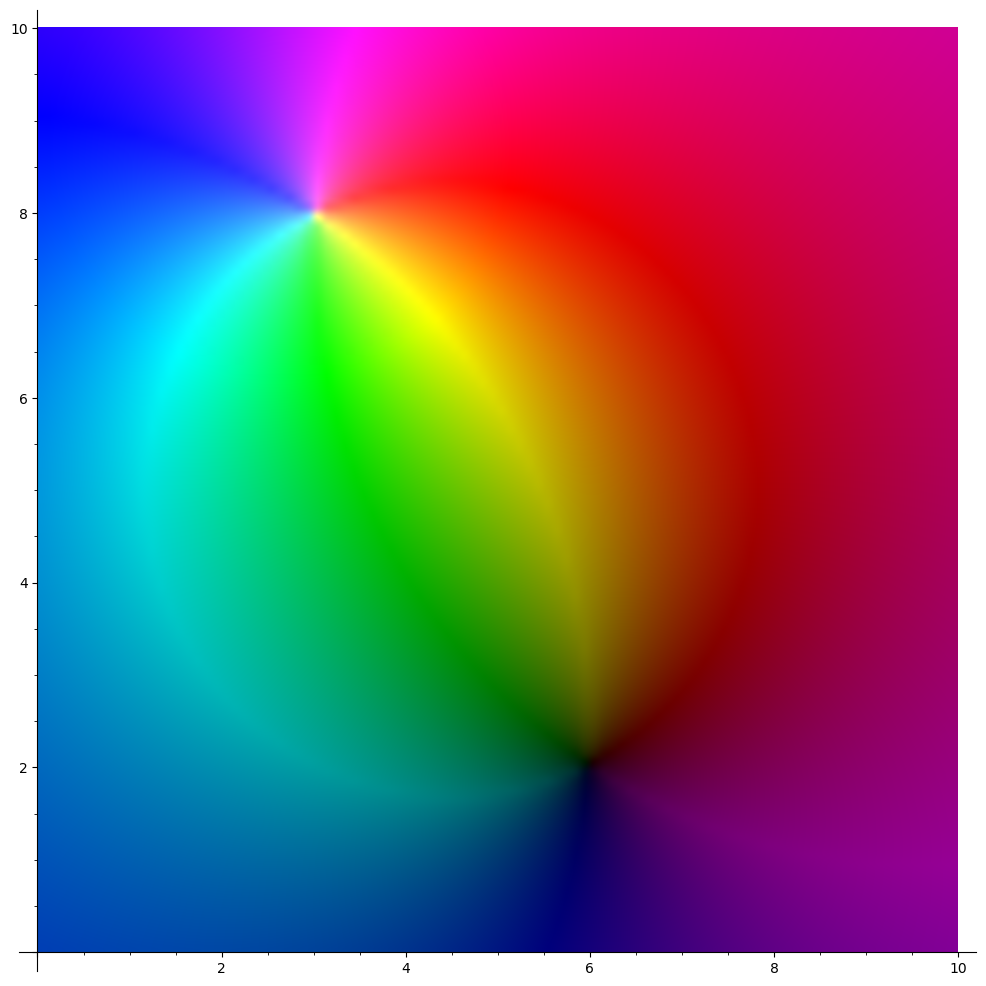
\includegraphics[width=9cm]{dc2}

\Problem
Consider the right figure.
It is the map
\[
    z \mapsto
    \frac{(a + bi) + (c + di)z}
    {(e + fi) + (g + hi)z}
\]
for some integers $(a, b, c, d, e, f, g, h)$
whose greatest common divisor is $1$, and $e$ and $f$ are positive.
Find those integers.
One point per correct integer after the first three correct integers.

\Problem
What conformal map maps the strip $1 < x + 2y < 2$
to the fan $1 < \arg z < 2$?

\Problem
A bijection is a map that is one-to-one (injective) and onto (surjective).
The map $\beta(z) = (z - i) / (z + i)$
maps the upper half plane $y > 0$ to the unit disk $r < 1$ bijectively.
(This is because, as $z$ is closer to $i$ than to $-i$,
we deduce that $|z - i|$ is smaller than $|z + i|$
and hence $|z - i| / |z + i| < 1$.)
Find the bijective map that maps the unit disk to itself,
$1$ to $1$, and $0$ to $1/2$.
There is only one such function.
Just find the function.
You don't have to prove uniqueness.

\Problem
Show that, for any complex number $z \neq 0$, the sum
$\sum_{m=1}^\infty m! z^m$ does not converge.

\Problem
The Riemann zeta function is defined as
\[\zeta(z) = \sum_{n=1}^\infty \frac1{n^z}\]
for all complex numbers $z$ with real part $> 1$.
We know that $\zeta(5 + 5i) \approx 0.?????9242554574 + 0.0119825174357425i$.
Find the missing digits.
One point per digit.

\Problem
Define $\kappa(z) = \cos(\sin(\cos(\sin(\cos(\sin(z))))))$.
Its second derivative at $0$ is $-0.?????0487021611$.
Find the missing digits.
One point per digit.

\Problem
Evaluate the imaginary part of the definite integral
$\int_\gamma \exp(z^2) dz$
where the curve $\gamma$ is a half circle
starting from $i$, passing through $1 + 2i$, and ending at $3i$.
The answer is $0.?????3215447094$.
Find the missing digits.
One point per digit.

\Problem
Let the curve $\delta(\tau)$ be $(r, \theta) = (2 \sin(2\tau), \tau)$
for $\tau$ from $0$ to $2\pi$.
Evaluate
\[ \oint_\delta \frac{\cos(z) dz}{z^8 - 1}.  \]

\Problem
The integral below is about $0.?????5218126363$.
Find the missing digits.
One point per digit.
\[ 2\int_0^\infty \frac{\cos(x) dx}{x^2 + \sqrt{2}} \]
Hint: It happens that $\cos(x)$ is the real part of $e^{ix}$.
So the problem is equivalent to the integral with $e^{ix}$ in the numerator,
and discarding the imaginary part after finishing.
Hint 2: Now integrating over the real line
is the limiting case of integrating over a long interval $[-M, M]$
and then the half circle passing $M$, $Mi$, and $Mi^2$.
How come we can add the half circle out of the thin air?
This is essentially because the integrand is $O(1/M^2)$.
For this question, just give me the evaluation of the integral.

\Problem
For this question, show me why the contribution
of the half circle tends to zero as $M$ tends to infinity.

\Problem
A function $f: \CC \setminus \{0\} \to \CC$
is holomorphic on the punctured plane $\CC \setminus \{0\}$.
It is said to have a removable singularity at $0$
if $\lim_{z \to 0} f(z)$ exists.
Now we try to ``patch'' the singularity at $0$
by defining
\[
    g(z) =
    \begin{cases}
        f(z), & z \neq 0 \\
        \lim_{z \to 0} f(z), & z = 0
    \end{cases}
\]
Show that $g$ is holomorphic on $\CC$.
Hint:
The problem is that $g$ is only continuous at $0$
and may not be differentiable at $0$.
After multiplying $g$ by something magic,
we can make it such that $(\text{magic} \cdot g)'(0)$ exists
and we know exactly its value.
And then we can divide the magical term and get back to $g$.
Do not cite big theorems.
We are trying to reproduce the proof.

\Problem 
$h: \DD \to \DD$ is holomorphic on the unit disk
$\DD = \{z \in \CC : |z| < 1\}$ such that $h(0) = 0$ and $|h(z)| \le 1$.
Show that $|h(z)| \le|z|$.

\Problem
A function $u: \RR^2 \to \RR$ is harmonic if its Laplacian
$(\partial^2 u/\partial x^2) + (\partial^2 u/\partial y^2)$
is zero everywhere.
For such a function, there exists another function $v: \RR^2 \to \RR$
such that $u + iv$, as a function in $(x, y)$,
is holomorphic in $z = x + yi$.
Try to express $v$ in terms of
some beautiful integral of something about $u$ (3 points).
Give a brief (about 50--100 words) explanation
why your $u + iv$ is holomorphic.

\Problem
For a sequence $a_0, a_1, a_2, \dotsc$, its generating function
is defined as $G(z) = a_0 + a_1 z + a_2 z^2 + \dotsb$.
Suppose that $a_0 = 0$ and $a_1 = 2$,
and that $4a_{j-1} - 4 a_j + a_{j+1} = 0$ for all $j$ that apply.
Find the generating function of this sequence (2 points).
Determine its radius of convergence (1 point).
Find the generating function of the filtered sequence
$a_0, 0, 0, a_3, 0, 0, a_6, 0, 0, a_9, \dotsc$ (2 points).

\Problem
For these three problems, one point per blank.
Answer on the answer sheet or blank paper.
By the \rule{3em}{0.4pt} theorem of \rule{3em}{0.4pt},
the polynomial $z^3 - 5iz + 20$ has \rule{3em}{0.4pt} roots.
Note that when $|z| > r =$ \rule{3em}{0.4pt} (an integer),
$|z^3|$ is greater than $|5iz| + |20|$,
which is greater than or equal to $|{-5iz + 20}|$
by the \rule{3em}{0.4pt} inequality.
So there is no root outside the disk of radius $r$.

\Problem
We can also see that there is
one root in the \rule{3em}{0.4pt} quadrant,
one in the \rule{3em}{0.4pt} quadrant, and
one in the \rule{3em}{0.4pt} quadrant.
Now using Newton's iteration $z_{n+1} = z_n - \frac{f(z_n)}{f'(z_n)}$,
we can quickly approximate the roots.

\Problem
The roots are, approximately,
$\rule{3em}{0.4pt}4673326721 + \rule{3em}{0.4pt}27885641441i$,
$\rule{3em}{0.4pt}34570814979 + \rule{3em}{0.4pt}3009971984i$, and
$\rule{3em}{0.4pt}1216245223 + \rule{3em}{0.4pt}5798536128i$.

\Problem
One point:
Write this down on the answer sheet or blank paper:
\emph{
I do not cheat on the exam,
I take photos of my exam paper after the exam time ends,
and I upload those photos to NTU COOL for future reference.
}

\clearpage

\section*{Complex Variable - Midterm Exam}

Name: \hrulefill Student ID: \hrulefill

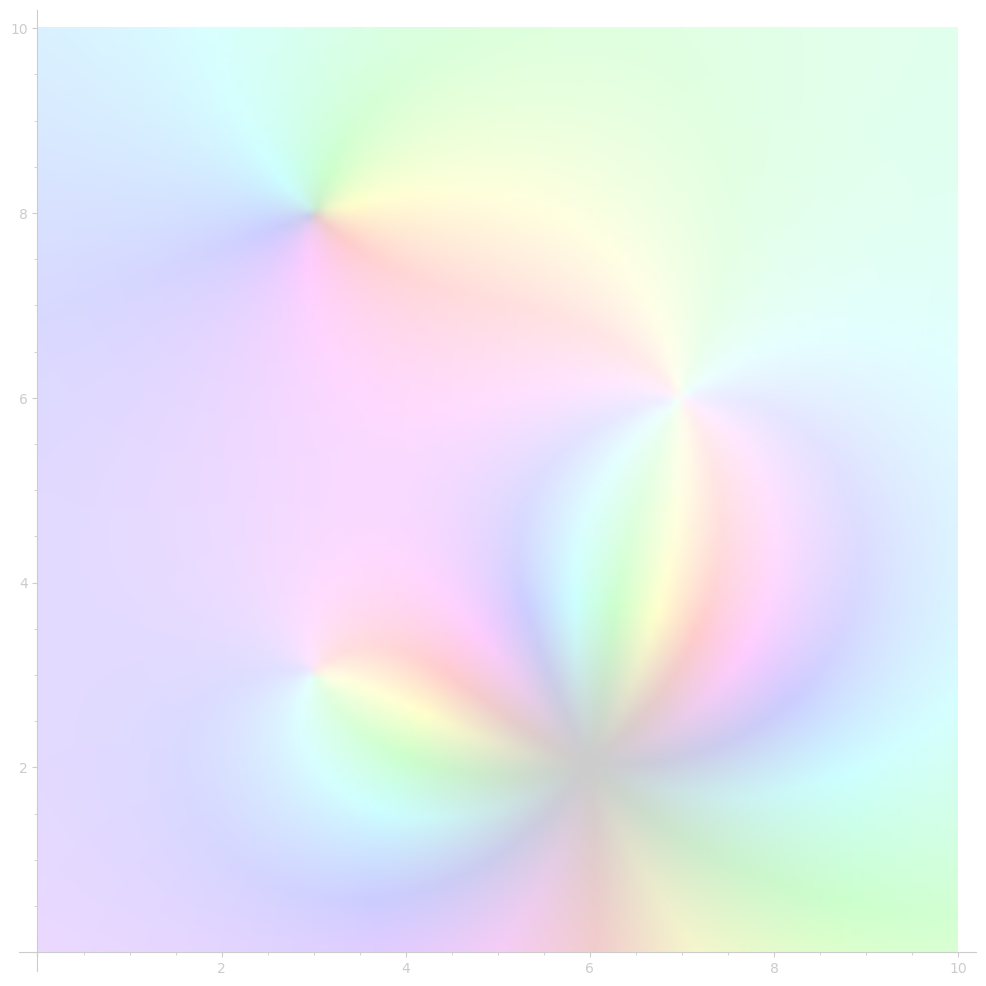
\includegraphics[width=9cm]{dc3}

\end{document}